% Combinatorial graphs
% Author: Rafael Villarroel
% Source: http://graphtheoryinlatex.blogspot.com/
\documentclass{article}
\usepackage{tikz}
\pagestyle{empty}
\usepackage{verbatim}

\begin{comment}
:Title: Combinatorial graphs
:Tags: Paths, Foreach, Graphs

Two fascinating graphs from the very interesting `Graph Theory in LaTeX`_ gallery.
The graphs are excellent examples of how flexible and powerful TikZ' path
constructs are. See the source code for more details.

*Update*: Fixed an error in the code for drawing Tutte's 8-cage graph.

:Author: Rafael Villarroel
:Source: The `Graph Theory in LaTeX`_ gallery

.. _Graph Theory in LaTeX: http://graphtheoryinlatex.blogspot.com/

\end{comment}

\begin{document}


% Define style for nodes
\tikzstyle{every node}=[circle, draw, fill=black!50,
                        inner sep=0pt, minimum width=4pt]
%  Tutte's 8-cage
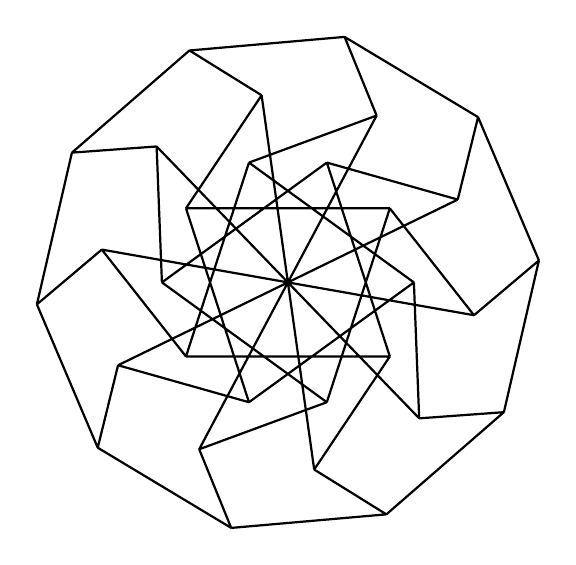
\begin{tikzpicture}[thick,scale=0.8]
    % The following path utilizes several useful tricks and features:
    % 1) The foreach statement is put inside a path, so all the edges
    %    will in fact be a the same path.
    % 2) The node construct is used to draw the nodes. Nodes are special
    %    in the way that they are drawn *after* the path is drawn. This
    %    is very useful in this case because the nodes will be drawn on
    %    top of the path and therefore hide all edge joins.
    % 3) Simple arithmetics can be used when specifying coordinates.
    \draw \foreach \x in {0,36,...,324}
    {
        (\x:2) node {}  -- (\x+108:2)
        (\x-10:3) node {} -- (\x+5:4)
        (\x-10:3) -- (\x+36:2)
        (\x-10:3) --(\x+170:3)
        (\x+5:4) node {} -- (\x+41:4)
    };
\end{tikzpicture}\quad
%
%
% The largest 3-regular graph of diameter 3
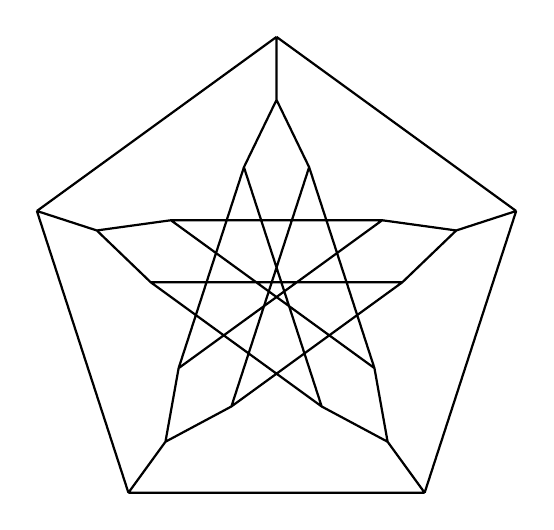
\begin{tikzpicture}[thick,scale=0.8]%
    \draw \foreach \x in {18,90,...,306} {
        (\x:4) node{} -- (\x+72:4)
        (\x:4) -- (\x:3) node{}
        (\x:3) -- (\x+15:2) node{}
        (\x:3) -- (\x-15:2) node{}
        (\x+15:2) -- (\x+144-15:2)
        (\x-15:2) -- (\x+144+15:2)
};
\end{tikzpicture}


\end{document}